\chapter{Classification and regression trees}\label{ch:cart}

\begin{remark}{Outline}
In this chapter, we present a unified framework in which we detail (single)
decision trees methods. In Section~\ref{sec:3:introduction}, we first give an
overview of the context in which these algorithms have been developed. In
Section~\ref{sec:3:tree-structured-models}, we proceed with a mathematical
presentation, introducing all necessary concepts and notations. The general
learning algorithm is then presented in Section~\ref{sec:3:induction} while
specific parts of the algorithm are discussed in finer details in
Sections~\ref{sec:3:assignment}, \ref{sec:3:stop}, \ref{sec:3:splitting-rules}.
As such, specific decision tree algorithms (e.g., CART, ID3 or C4.5) are described as
specializations of the general framework presented here.
\end{remark}

\section{Introduction}
\label{sec:3:introduction}

Since always, artificial intelligence has been driven by the ambition to
understand and uncover complex relations in data. That is, to find models that
can not only produce accurate predictions, but also be used to extract
knowledge in an intelligible way. Guided with this twofold objective, research
in machine learning has given rise to extensive bodies of works in a myriad of
directions. Among all of them however, tree-based methods stand as one of
the most effective and useful method, capable to produce both reliable and
understandable results, on mostly any kind of data.

Historically, the appearance of \textit{decision trees} is due to
\citet{morgan:1963}, who first proposed a tree-based method called
\textit{automatic interaction detector} (AID) for handling multi-variate
non-additive effects in the context of survey data. Building upon AID,
methodological improvements and computer programs for exploratory analysis were
then proposed in the following years by several
authors~\citep{sonquist:1970,messenger:1972,gillo:1972,sonquist:1974}. Without
contest however, the principal investigators that have driven research on the modern
methodological principles are \citet{breiman:1978a,breiman:1978b},
\citet{friedman:1977,friedman:1979} and \citet{quinlan:1979,quinlan:1986} who
simultaneously and independently proposed very close algorithms for the
induction of tree-based models. Most notably, the unifying work of
\citet{breiman:1984}, later complemented with the work of \citet{quinlan:1993},
have set decision trees into a simple and consistent methodological framework,
which largely contributed in making them easy to understand and easy to use by
a large audience.

As we will explore in further details all throughout this work, the success
of decision trees (and by extension, of all tree-based methods) is explained
by several factors that make them quite attractive in practice:
\begin{itemize}
\item Decision trees are non-parametric. They can model arbitrarily complex relations between inputs and outputs, without any a priori assumption;
\item Decision trees handle heterogeneous data (ordered or categorical variables, or a mix of both);
\item Decision trees intrinsically implement feature selection, making them robust to irrelevant or noisy variables;
\item Decision trees are robust to outliers or errors in labels;
\item Decision trees are easily interpretable, even for non-statistically oriented users.
\end{itemize}

Most importantly, decision trees are at the foundation of many modern and
state-of-the-art algorithms, including forests of randomized trees (on which
this work is about, see Chapter~\ref{ch:forest}) or boosting
methods~\citep{freund:1995,friedman:2001}, where they are used as building
blocks for composing larger models. Understanding all algorithmic details of
single decision trees is therefore a mandatory prerequisite for an in-depth
analysis of these methods.


\section{Tree structured models}
\label{sec:3:tree-structured-models}

When the output space is a finite set of values, like in classification where
${\cal Y} = \{c_1, c_2, ..., c_J\}$, another way of looking at a supervised
learning problem is to notice that $Y$ defines a partition over the universe
$\Omega$, that is
\begin{equation}
\Omega = \Omega_{c_1} \cup \Omega_{c_2} \cup \dots \cup \Omega_{c_J},
\end{equation}
where $\Omega_{c_k}$ is the of set objects for which $Y$ has value $c_k$.
Similarly, a classifier $\varphi$ can also be regarded as a partition of the
universe $\Omega$ since it defines an approximation $\widehat{Y}$ of $Y$.
This partition however is defined on the input space ${\cal X}$ rather
that directly on $\Omega$, that is
\begin{equation}\label{eqn:3:partition}
{\cal X} = {\cal X}^\varphi_{c_1} \cup {\cal X}^\varphi_{c_2} \cup ... \cup {\cal X}^\varphi_{c_J},
\end{equation}
where
${\cal X}^\varphi_{c_k}$ is the set of description vectors $\mathbf{x} \in {\cal X}$ such that
$\varphi(\mathbf{x}) = c_k$. Accordingly, learning a classifier can
be restated as learning a partition of ${\cal X}$ matching as closely as
possible the best possible partition, i.e., the one engendered by the Bayes model $\varphi_B$ over ${\cal X}$:
\begin{equation}\label{eqn:3:partition}
{\cal X} = {\cal X}^{\varphi_B}_{c_1} \cup {\cal X}^{\varphi_B}_{c_2} \cup ... \cup {\cal X}^{\varphi_B}_{c_J}.
\end{equation}

\begin{remark}{Partitioning with noise}
Notice that when $Y$ cannot be univocally determined given $X=\mathbf{x}$,
e.g., when there is noise on $Y$, then there may exist two distinct objects from the universe $\Omega$ such
that their representations $\mathbf{x}_1$ and $\mathbf{x}_2$ in the input space
are equal, yet such that the corresponding output values $y_1$ and $y_2$ are different.
In other words, the subsets
\begin{equation}
{\cal X}^\Omega_{c_k} = \{ \mathbf{x}_i | i \in \Omega, Y=c_k \}
\end{equation}
may not be disjoints.
By contrast, since $\varphi$ defines a function from ${\cal X}$ to ${\cal Y}$,
any input $\mathbf{x} \in {\cal X}$ is mapped to exactly one output value $y \in
{\cal Y}$ and the subsets ${\cal X}^\varphi_{c_k}$ are therefore necessarily
disjoints, which means that no model will ever perfectly predict the true output
value in all cases. As discussed in Section~\ref{sec:2:bayes-model}, this
limitation is unavoidable and can in fact be viewed as the cause of the residual error.
\end{remark}

From a geometrical point of view, the principle of tree structured models is
beautifully simple. It consists in approximating the partition of the Bayes
model by recursively partitioning the input space ${\cal X}$ into subspaces and
then assign constant prediction values $\widehat{y}\in{\cal Y}$ to all objects
$\mathbf{x}$ within each terminal subspace. To make things clearer, let us
first define the following concepts:

\begin{definition}
A \emph{tree} is a graph $G=(V,E)$ in which any two vertices (or \emph{nodes})
are connected by exactly one path.
\end{definition}

\begin{definition}
A \emph{rooted tree} is a tree in which one of the nodes has been designated as
the \emph{root}. In our case, we additionally assume that a rooted tree is a
\emph{directed} graph, where all edges are directed away from the root.
\end{definition}

\begin{definition}
If there exists an edge from $t_1$ to $t_2$ (i.e., if $(t_1, t_2)\in E$) then
node $t_1$ is said to be the \emph{parent} of node $t_2$ while node $t_2$ is
said to be a \emph{child} of node $t_1$.
\end{definition}

\begin{definition}
In a rooted tree, a node is said to be \emph{internal} if it has one or more
children and \emph{terminal} if it has no children. Terminal nodes are also
known as \emph{leaves}.
\end{definition}

\begin{definition}
A \emph{binary tree} is a rooted tree where all internal nodes exactly
have two children.
\end{definition}

In those terms, a \textit{tree-structured model} (or \textit{decision tree})
can be defined as a model $\varphi: {\cal X} \mapsto {\cal Y}$ represented by a
rooted tree (often binary, but not necessarily), where any node $t$ represents
a subspace ${\cal X}_t \subseteq {\cal X}$ of the input space, with the root
node $t_0$ corresponding to ${\cal X}$ itself. Internal nodes $t$ are labeled with a
\textit{split} $s_t$ (taken from a set of questions ${\cal Q}$) dividing the
space ${\cal X}_t$ they each represent into disjoint subspaces respectively
corresponding to each of their children. For instance, the set of all binary
splits is the set ${\cal Q}$ of questions $s$ of the form \textit{``Is
$\mathbf{x} \in {\cal X}_A?$''}, where ${\cal X}_A \subset {\cal X}$ is some
subset of the input space. Any split $s$ of this form divides ${\cal X}_t$ into
two subspaces respectively corresponding to ${\cal X}_t \cap {\cal X}_A$ for
the left child of $t$ and to ${\cal X}_t \cap ({\cal X}\setminus{\cal X}_A)$
for the right child of $t$. Terminal nodes are labeled with a best guess value
$\widehat{y}_t \in {\cal Y}$ of the output variable. If $\varphi$ is a
classification tree, then $\widehat{y}_t \in \{ c_1, ..., c_J \}$ while if
$\varphi$ is a regression tree, then $\widehat{y}_t \in \mathbb{R}$. As such,
the predicted output value $\varphi(\mathbf{x})$
is the label of the leaf reached by the instance $\mathbf{x}$ when it is propagated through
the tree by following the splits $s_t$ (see Algorithm~\ref{algo:prediction}).

\begin{algorithm}\label{algo:prediction}
Prediction of the output value $\widehat{y} =\varphi(\mathbf{x})$ in a decision tree.
\textnormal{
\begin{algorithmic}[1]
\Function{Predict}{$\varphi, \mathbf{x}$}
    \State $t = t_0$
    \While{$t$ is not a terminal node}
        \State $t =$ the child node $t'$ of $t$ such that $\mathbf{x} \in {\cal X}_{t'}$
    \EndWhile
    \State \Return $\widehat{y}_t$
\EndFunction
\end{algorithmic}
}
\end{algorithm}

\begin{figure}
    \centering
    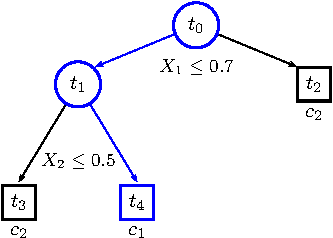
\includegraphics[scale=1.0]{figures/ch3_tree.pdf}
    \caption{A decision tree $\varphi$ built for a binary classification
             problem from an input space ${\cal X}=[0,1]\times[0,1]$.
             (Figure inspired from \citet{breiman:1984}.)}
    \label{fig:3:tree}
\end{figure}

\begin{figure}
    \centering
    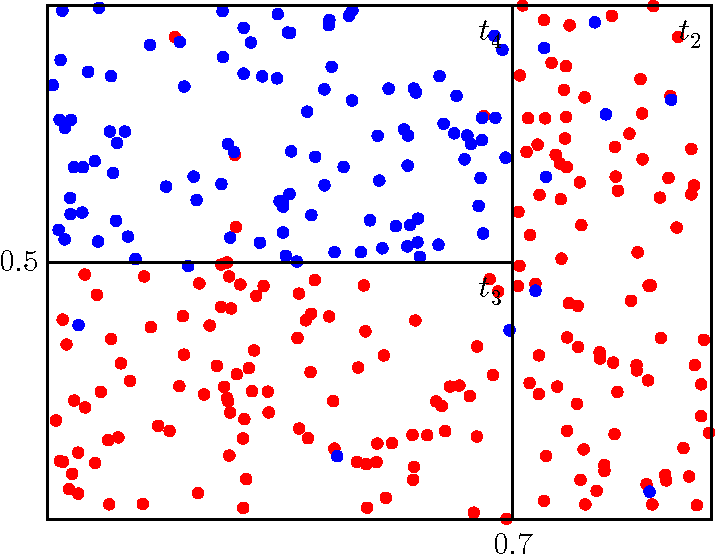
\includegraphics[width=0.9\textwidth]{figures/ch3_partition.pdf}
    \caption{Partition of ${\cal X}$ induced by the decision tree $\varphi$ into homogeneous subspaces.
             Blue dots correspond to objects of class $c_1$ while red dots correspond
             to objects of class $c_2$. (Figure inspired from \citet{breiman:1984}.)}
    \label{fig:3:partition}
\end{figure}

As an example, Figure~\ref{fig:3:tree} illustrates a decision tree $\varphi$
made of five nodes and partitioning the input space ${\cal X} = {\cal X}_1
\times {\cal X}_2 = [0;1] \times [0; 1]$ for a binary classification problem
(where ${\cal Y}=\{ c_1, c_2 \}$). Node $t_0$ is the root node and corresponds
to the whole input space ${\cal X}_{t_0} = {\cal X}$. It is labeled with the binary
split $X_1 \leq 0.7$ (i.e., the question \textit{``Is $X_1 \leq 0.7$?''}) which divides ${\cal X}_{t_0}$ into two disjoint subsets
${\cal X}_{t_1} \cup {\cal X}_{t_2}$. The first set corresponds to its left
child $t_1$ and represents the set of all input vectors $\mathbf{x} \in {\cal
X}_0$ such that $x_1 \leq 0.7$. Similarly, the second set corresponds to its
right child $t_2$ and represents the set of all input vectors $\mathbf{x} \in
{\cal X}_{t_0}$ such that $x_1 > 0.7$. Likewise, $t_1$ is labeled with the
split $X_2 \leq 0.5$ which further divides ${\cal X}_{t_1}$ into two disjoint
subsets ${\cal X}_{t_3} \cup {\cal X}_{t_4}$ respectively corresponding the
sets of all input vectors $\mathbf{x} \in {\cal X}_{t_1}$ such that $x_2 \leq
0.5$ (resp. $x_2 > 0.5$). Terminal nodes $t_2$, $t_3$ and $t_4$ are represented
by squares labeled with an output value $\widehat{y}_t$. They form together a
partition (as defined by Equation~\ref{eqn:3:partition}) of ${\cal X}$, where
each set $\widehat{{\cal X}_{c_k}}$ is obtained from the union of the subspaces
${\cal X}_t$ of all terminal nodes $t$ such that $\widehat{y}_t = c_k$. In this
case, $\widehat{{\cal X}_{c_1}} = {\cal X}_{t_4}$ while $\widehat{{\cal
X}_{c_2}} = {\cal X}_{t_2} \cup {\cal X}_{t_3}$. As shown in
Figure~\ref{fig:3:partition}, the partition engendered by  $\varphi$ on ${\cal
X}$ divides the input space into subspaces that are more and more class
homogeneous, starting from ${\cal X}$ at the root node,  then ${\cal X}_{t_1}
\cup {\cal X}_{t_2}$ at the second level of tree and finally $({\cal X}_{t_3}
\cup {\cal X}_{t_4})\cup {\cal X}_{t_2}$ at the leaves.  As we will explore in
Section~\ref{sec:3:splitting-rules}, the partition is in this case made of
rectangles because of the nature of the splits $s_t \in {\cal Q}$ dividing the nodes.
Predictions are made by propagating instances through the tree and using as
output value the value labeling the terminal nodes in which they fall
into. For example, an object $\mathbf{x}=(x_1=0.2, x_2=0.7)$ falls into $t_4$
and therefore $\varphi(\mathbf{x}) = \widehat{y}_{t_4} = c_1$.

Finally, let us note that from a graph theory point of view, decision trees
belong to a larger family of methods known as \textit{induction
graphs}~\citep{zighed:2000}. In this more general framework, the structure is a
directed acyclic graph, which allows for nodes to be both divided and
recombined.

\section{Induction of decision trees}
\label{sec:3:induction}

Learning a decision tree ideally amounts to determine the tree structure which
produces the partition which is closest to the partition engendered by $Y$ over
${\cal X}$. Since it is unknown however, the construction of a decision tree is usually
driven instead with the objective of finding a model which partitions the
learning set ${\cal L}$ as best as possible. Among all decision trees $\varphi
\in {\cal H}$ however, there may exist several of them that explain ${\cal L}$
equally best. Following Occam's Razor principles~\citep{blumer:1987} of preferring the explanation
which makes as few assumptions as possible, that is to favor the simplest
solution that fits the data, learning a decision tree from ${\cal L}$ is
usually restated as finding the smallest tree $\varphi^*$ (in terms of internal nodes) minimizing its
resubstitution estimate $\overline{E}(\varphi^*, {\cal L})$. While this
assumption makes sense from a generalization point of view, it also makes
sense regarding interpretability. A decision tree which is small is easier
to understand than a large and complex tree.

As shown by \citet{hyafil:1976} however, finding the smallest tree $\varphi^*$
that minimizes its resubstitution estimate is an NP-complete problem. As a
consequence, under the assumption that $P \neq NP$, there exists no efficient
algorithm for finding $\varphi^*$, thereby suggesting that finding efficient heuristics
for constructing near-optimal decision trees is the best solution to keep computation
requirements within realistic boundaries.

Following the framework of \citet{breiman:1984}, let us broadly define an
\textit{impurity} measure $i(t)$ as a function that evaluates the goodness of
any node $t$ (we delay to Section~\ref{sec:3:splitting-rules} for a more
precise definition). Let assume that the smaller $i(t)$, the \textit{purer} the
node and the better the predictions $\widehat{y}_t(\mathbf{x})$ for all
$\mathbf{x} \in {\cal L}_t$, where ${\cal L}_t$ is the subset of learning
samples falling into $t$, that is all $(\mathbf{x}, y) \in {\cal L}$ such that
$\mathbf{x} \in {\cal X}_t$.
Starting from a single node representing the whole learning set  ${\cal L}$,
near-optimal decision trees can then be grown greedily by iteratively dividing
nodes into purer nodes. That is, by iteratively  dividing into smaller subsets the
subsets of ${\cal L}$ represented by the nodes, until all terminal nodes cannot
be made purer, hence guaranteeing near-optimal predictions over ${\cal L}$. The
greedy assumption to make the resulting tree as small as possible, thereby
seeking for good generalization, is then to divide each node $t$ using the
split $s^*$ that locally maximizes the decrease of impurity of the resulting child nodes.

Formally, the decrease of impurity of a binary split $s$ is defined as follows:
\begin{definition}\label{def:impurity-decrease}
The \emph{impurity decrease} of a binary split $s \in {\cal Q}$ dividing node $t$ into
a left node $t_L$ and a right node $t_R$ is
\begin{equation}
\Delta i(s, t) = i(t) - p_L i(t_L) - p_R i(t_R)
\end{equation}
where $p_L$ (resp., $p_R$) is the proportion $\tfrac{N_{t_L}}{N_t}$ (resp., $\tfrac{N_{t_R}}{N_t}$)
of learning samples from ${\cal L}_t$ going to $t_L$ (resp., to $t_R$) and where $N_t$
is the size of the subset ${\cal L}_t$.
\end{definition}

On the basis of this concept, a general greedy procedure for the induction of
decision trees can now be described formally as outlined in
Algorithm~\ref{algo:induction}. Note that for the sake of clarity,
Algorithm~\ref{algo:induction} is formulated in terms of binary splits.
However, as we will explore later in Section~\ref{sec:3:splitting-rules}, it
generalizes naturally to $n$-ary splits.

\begin{algorithm}\label{algo:induction}
Greedy induction of a binary decision tree.
\textnormal{
\begin{algorithmic}[1]
\Function{BuildDecisionTree}{${\cal L}$}
    \State Create a decision tree $\varphi$ with root node $t_0$
    \State Create an empty stack $S$ of \emph{open} nodes $(t, {\cal L}_t)$
    \State $S$\Call{.push}{($t_0, {\cal L}$)}
    \While{$S$ is not empty}
        \State $t, {\cal L}_t =$ $S$\Call{.pop}{~}
        \If{the stopping criterion is met for $t$}\label{algo:induction:stop}
            \State $\widehat{y}_{t} =$ some constant value\label{algo:induction:terminal}
        \Else
            \State Find the split on ${\cal L}_t$ that maximizes impurity decrease $$s^* = \argmax_{s \in {\cal Q}} \Delta i(s, t)$$ \label{algo:induction:split}
            \State Partition ${\cal L}_t$ into ${\cal L}_{t_L} \cup {\cal L}_{t_R}$ according to $s^*$
            \State Create the left child node $t_L$ of $t$
            \State Create the right child node $t_R$ of $t$
            \State $S$\Call{.push}{($t_R, {\cal L}_{t_R}$)}
            \State $S$\Call{.push}{($t_L, {\cal L}_{t_L}$)}
        \EndIf
    \EndWhile
    \State \Return $\varphi$
\EndFunction
\end{algorithmic}
}
\end{algorithm}

The rest of this chapter is now dedicated to a detailed discussion of specific
parts of Algorithm~\ref{algo:induction}. Section~\ref{sec:3:assignment}
discusses assignment rules for terminal nodes
(Line~\ref{algo:induction:terminal} of Algorithm~\ref{algo:induction}) while
Section~\ref{sec:3:stop} outlines stopping criteria for deciding when a node
becomes terminal (Line~\ref{algo:induction:stop} of
Algorithm~\ref{algo:induction}). Section~\ref{sec:3:splitting-rules} then
presents families ${\cal Q}$ of splitting rules, impurity criteria $i(t)$ to
evaluate the goodness of splits and strategies for
finding the best split $s^* \in {\cal Q}$ (Line~\ref{algo:induction:split} of
Algorithm~\ref{algo:induction}). As we will see, the crux of the problem is in
finding good splits and in knowing when to stop splitting.


\section{Assignment rules}
\label{sec:3:assignment}

Let us assume that node $t$ has been declared terminal given some stopping
criterion (See next Section~\ref{sec:3:stop}). The next step
(Line~\ref{algo:induction:terminal} of Algorithm~\ref{algo:induction}) in the
induction procedure is to label $t$ with a constant value $\widehat{y}_t$ to
be used as a prediction of the output variable $Y$. As such, node $t$ can  be
regarded as a simplistic model defined locally on ${\cal X}_t \times {\cal Y}$
and producing the same output value $\widehat{y}_t$ for all possible input
vectors falling into $t$.

Let us first notice that, for a tree $\varphi$ of \textit{fixed} structure,
minimizing the global generalization error is strictly equivalent to minimizing
the local generalization error of each simplistic model in the terminal nodes.
Indeed,
\begin{align}
Err_{\cal L}(\varphi) &= \mathbb{E}_{X,Y} \{ L(Y, \varphi(X)) | {\cal L} \} \nonumber \\
                      &= \sum_{t \in \widetilde{\varphi}} P(X \in {\cal X}_t) \mathbb{E}_{X,Y|t} \{ L(Y, \widehat{y}_t) | {\cal L} \} \label{eqn:assignment-generalization}
\end{align}
where $\widetilde{\varphi}$ denotes the set of terminal nodes in $\varphi$
and where the inner expectation\footnote{The joint expectation of $X$ and $Y$
is taken over all objects $i \in \Omega$ such that $\mathbf{x}_i \in {\cal X}_t$.}
is the local generalization error of the model at node $t$. In this later form,
a model which minimizes $Err_{\cal L}(\varphi)$ is a model which minimizes the inner
expectation leaf-wise. Learning the best possible decision tree (of
fixed structure) therefore simply amounts to find the best constants
$\widehat{y}_t$ at each terminal node.

\subsection{Classification}

When $L$ is the zero-one loss, the inner expectation in Equation~\ref{eqn:assignment-generalization}
is minimized by the plurality rule:
\begin{align}
\widehat{y}_t^* &= \argmin_{c \in {\cal Y}} \mathbb{E}_{X, Y|t}\{ 1(Y, c) | {\cal L} \} \nonumber \\
                &= \argmin_{c \in {\cal Y}} P(Y \neq c | X \in {\cal X}_t) \nonumber \\
                &= \argmax_{c \in {\cal Y}} P(Y = c | X \in {\cal X}_t)\label{eqn:assignment-classification}
\end{align}
Put otherwise, the generalization error of $t$ is minimized by predicting
the class which is the most likely for the samples in the subspace of $t$.
Note that if the maximum is achieved by two or more different classes, then
$\widehat{y}_t^*$ is assigned arbitrarily as any one of the maximizing classes.

Equation~\ref{eqn:assignment-classification} cannot be solved without the
probability distribution $P(X, Y)$. However, its solution can be approximated
by using estimates of the local generalization error. Let $N_t$ denotes the
number of objects in ${\cal L}_t$ and let $N_{ct}$ denotes the number of
objects of class $c$ in ${\cal L}_t$. Then, the proportion
$\tfrac{N_{ct}}{N_t}$ can be interpreted as the estimated
probability\footnote{Lower case $p$ denotes an estimated probability while
upper case $P$ denotes a theoretical probability.} $p(Y=c|X\in{\cal X}_t)$
(shortly denoted $p(c|t)$) of class $c$ in $t$ and therefore be used to solve
Equation~\ref{eqn:assignment-classification}:
\begin{align}\label{eqn:assignement-classification-approx}
\widehat{y}_t &= \argmin_{c \in {\cal Y}} 1 - p(c | t) \nonumber \\
              &= \argmax_{c \in {\cal Y}} p(c | t)
\end{align}

Similarly, let us also define the proportion $\tfrac{N_t}{N}$ as the estimated
probability $p(X \in {\cal X}_t)$ (shortly denoted $p(t)$). Plugging this
estimate into Equation~\ref{eqn:assignment-generalization} and approximating
the local generalization error with $1 - p(\widehat{y}_t | t)$ as done above, it follows:
\begin{align}
\widehat{Err}_{\cal L}(\varphi) &= \sum_{t \in \widetilde{\varphi}} p(t) (1 - p(\widehat{y}_t | t)) \nonumber \\
    &= \sum_{t \in \widetilde{\varphi}} \frac{N_t}{N} (1 - \frac{N_{{\widehat{y}_t}t}}{N_t}) \nonumber \\
    &= \frac{1}{N} \sum_{t \in \widetilde{\varphi}} N_t - N_{{\widehat{y}_t}t} \nonumber \\
    &= \frac{1}{N} \sum_{t \in \widetilde{\varphi}} \sum_{\mathbf{x}, y \in {\cal L}_t} 1(y \neq \widehat{y}_t) \nonumber \\
    &= \frac{1}{N} \sum_{\mathbf{x}, y \in {\cal L}} 1(y \neq \varphi(t)) \nonumber \\
    &= \widehat{Err}_{\cal L}^\text{train}(\varphi) \label{eqn:train-error-tree}
\end{align}
Accordingly, approximating Equation~\ref{eqn:assignment-generalization}
through local probability estimates computed from class proportions in
${\cal L}_t$ reduces to the resubstitution estimate of $\varphi$
(Equation~\ref{eqn:training-error}). In other words, assignment
rule~\ref{eqn:assignement-classification-approx} in fact minimizes the
resubstitution estimate rather than the true
generalization error.

An important property of assignment
rule~\ref{eqn:assignement-classification-approx} is that the more one splits a terminal node \textit{in
any way}, the smaller the resubstitution estimate $\smash{\widehat{Err}_{\cal
L}^\text{train}(\varphi)}$ becomes.

\begin{proposition}\label{prop:any-split-reduce-classification}
For any non-empty split of a terminal node $t \in \widetilde{\varphi}$ into $t_L$ and
$t_R$, resulting in a new tree $\varphi^\prime$ where $\widehat{y}_{t_L}$ and $\widehat{y}_{t_R}$
are assigned with rule~\ref{eqn:assignement-classification-approx}, $$\widehat{Err}_{\cal
L}^\text{train}(\varphi) \geq \widehat{Err}_{\cal
L}^\text{train}(\varphi^\prime)$$ with equality if $\widehat{y}_t =
\widehat{y}_{t_L} = \widehat{y}_{t_R}$.
\end{proposition}

\begin{proof}
\begin{align*}
\widehat{Err}_{\cal L}^\text{train}(\varphi) &\geq \widehat{Err}_{\cal L}^\text{train}(\varphi^\prime)  \\
\sum_{t \in \widetilde{\varphi}} p(t) (1 - p(\widehat{y}_t | t)) &\geq \sum_{t \in \widetilde{\varphi^\prime}} p(t) (1 - p(\widehat{y}_t | t)) \\
p(t) (1 - p(\widehat{y}_t | t)) &\geq p(t_L) (1 - p(\widehat{y}_{t_L} | t_L)) + p(t_R) (1 - p(\widehat{y}_{t_R} | t_R))\\
\frac{N_t}{N} (1 - \max_{c \in {\cal Y}} \frac{N_{ct}}{N_t}) &\geq \frac{N_{t_L}}{N} (1 - \max_{c \in {\cal Y}} \frac{N_{ct_L}}{N_{t_L}}) + \frac{N_{t_R}}{N} (1 - \max_{c \in {\cal Y}} \frac{N_{ct_R}}{N_{t_R}}) \\
N_t - \max_{c \in {\cal Y}} N_{ct} &\geq N_{t_L} - \max_{c \in {\cal Y}} N_{ct_L} + N_{t_R} - \max_{c \in {\cal Y}} N_{ct_R} \\
\max_{c \in {\cal Y}} N_{ct} &\leq \max_{c \in {\cal Y}} N_{ct_L} + \max_{c \in {\cal Y}} N_{ct_R} \\
\max_{c \in {\cal Y}} (N_{ct_L} + N_{ct_R}) &\leq \max_{c \in {\cal Y}} N_{ct_L} + \max_{c \in {\cal Y}} N_{ct_R}
\end{align*}
Which is true since $\max_{c \in {\cal Y}} N_{ct_L}$ (resp., $t_R$) is
necessarily greater or equal to the left term $N_{ct_L}$ (resp., to right term
$N_{ct_R}$) in the left-hand side of the equation. Equality holds if the
majority classes are the same in $t$, $t_L$ and $t_R$.
\end{proof}

As a corollary of Proposition~\ref{prop:any-split-reduce-classification}, the
resubstitution estimate is minimal when terminal nodes can no longer be
divided.  In particular, it is equal to zero if the tree can be \textit{fully
developed}, that is if terminal nodes can be divided until they all contain
exactly one object from ${\cal L}$. Based on this result, we will show however
in Section~\ref{sec:3:criteria} why using the resubstitution estimate to
evaluate the goodness of a split $s$ has serious defects for classification.

\subsection{Regression}

When $L$ is the squared error loss, the inner expectation in
Equation~\ref{eqn:assignment-generalization}
is minimized by the expectation of $Y$ in $t$:
\begin{align}
\widehat{y}_t^* &= \argmin_{\widehat{y} \in {\cal Y}} \mathbb{E}_{X, Y|t}\{ (Y - \widehat{y})^2 | {\cal L} \} \nonumber \\
                &= \mathbb{E}_{X, Y|t} \{ Y \} \label{eqn:assignment-regression}
\end{align}

Again, Equation~\ref{eqn:assignment-regression} cannot be solved
without the probability distribution $P(X, Y)$. However, its solution can
approximated using estimates of the local generalization error:
\begin{align}\label{eqn:assignement-regression-approx}
\widehat{y}_t   &= \argmin_{\widehat{y} \in {\cal L}} \frac{1}{N_t} \sum_{\mathbf{x}, y \in {\cal L}_t} (y - \widehat{y})^2 \nonumber \\
                &= \frac{1}{N_t} \sum_{\mathbf{x}, y \in {\cal L}_t} y
\end{align}

As in classification, using $p(t)$ as estimate of $P(X \in {\cal X}_t)$ and approximating
the local generalization error with $\tfrac{1}{N_t} \sum_{\mathbf{x}, y \in {\cal
L}_t} (y - \widehat{y}_t)^2$ as done above, one can show that
Equation~\ref{eqn:assignment-generalization} reduces to the resubstitution estimate of $\varphi$, thereby
indicating that assignment rule~\ref{eqn:assignement-regression-approx}
also minimizes the training error rather the true generalization error.

Most importantly, one can also show that assignment rule~\ref{eqn:assignement-regression-approx}
behaves in the same way as \ref{eqn:assignement-classification-approx}. The
more one splits a terminal node in any way, the smaller the resubstitution estimate $\smash{\widehat{Err}_{\cal
L}^\text{train}(\varphi)}$ becomes.

\begin{proposition}\label{prop:any-split-reduce-regression}
For any non-empty split of a terminal node $t \in \widetilde{\varphi}$ into $t_L$ and
$t_R$, resulting in a new tree $\varphi^\prime$ where $\widehat{y}_{t_L}$ and $\widehat{y}_{t_R}$
are assigned with rule~\ref{eqn:assignement-regression-approx}, $$\widehat{Err}_{\cal
L}^\text{train}(\varphi) \geq \widehat{Err}_{\cal
L}^\text{train}(\varphi^\prime)$$ with equality if $\widehat{y}_{t_L} = \widehat{y}_{t_R} = \widehat{y}_t$.
\end{proposition}

\begin{proof}
\begin{align*}
\widehat{Err}_{\cal L}^\text{train}(\varphi) &\geq \widehat{Err}_{\cal L}^\text{train}(\varphi^\prime)  \\
\sum_{t \in \widetilde{\varphi}} p(t) (\frac{1}{N_t} \sum_{\mathbf{x}, y \in {\cal L}_t} (y - \widehat{y}_t)^2) &\geq \sum_{t \in \widetilde{\varphi^\prime}} p(t) (\frac{1}{N_t} \sum_{\mathbf{x}, y \in {\cal L}_t} (y - \widehat{y}_t)^2) \\
\sum_{\mathbf{x}, y \in {\cal L}_t} (y - \widehat{y}_t)^2 &\geq \sum_{\mathbf{x}, y \in {\cal L}_{t_L}} (y - \widehat{y}_{t_L})^2 + \sum_{\mathbf{x}, y \in {\cal L}_{t_R}} (y - \widehat{y}_{t_R})^2 \\
N_t \widehat{y}_t^2 &\leq N_{t_L} \widehat{y}_{t_L}^2 + N_{t_R} \widehat{y}_{t_R}^2 \\
\frac{1}{N_t} (\sum_{\mathbf{x}, y \in {\cal L}_{t}} y)^2 &\leq \frac{1}{N_{t_L}} (\sum_{\mathbf{x}, y \in {\cal L}_{t_L}} y)^2 + \frac{1}{N_{t_R}} (\sum_{\mathbf{x}, y \in {\cal L}_{t_R}} y)^2
\end{align*}
For simplifying, let us denote $s(t) = \sum_{\mathbf{x}, y \in {\cal L}_{t}} y = N_t \widehat{y}_t$
the sum of the output values in $t$. Remark that $s(t) = s(t_L) + s(t_R)$. It comes:
\begin{align*}
\frac{s(t)^2}{N_t} &\leq \frac{s(t_L)^2}{N_{t_L}} + \frac{s(t_R)^2}{N_{t_R}} \\
\frac{(s(t_L) + s(t_R))^2}{N_{t_L} + N_{t_R}} &\leq \frac{s(t_L)^2}{N_{t_L}} + \frac{s(t_R)^2}{N_{t_R}} \\
\frac{(s(t_L) N_{t_R} - s(t_R) N_{t_L})^2}{N_{t_L} N_{t_R} (N_{t_L} + N_{t_R})} &\geq 0
\end{align*}
Which is necessary true since the numerator is non-negative and the denominator is
strictly positive. Equality holds if $s(t_L) N_{t_R} = s(t_R) N_{t_L}$, that is if $\widehat{y}_{t_L} = \widehat{y}_{t_R}$.
\end{proof}

As for Proposition~\ref{prop:any-split-reduce-classification}, a corollary of Proposition~\ref{prop:any-split-reduce-regression}
is that the resubstitution estimate is minimal when terminal nodes can no longer be divided.


\section{Stopping criteria}
\label{sec:3:stop}

As we have shown through Propositions~\ref{prop:any-split-reduce-classification}
and \ref{prop:any-split-reduce-regression}, the deeper a
decision tree, the smaller its training estimate, and the better we think it
is. As discussed in Section~\ref{sec:2:model-selection} however, increasing
model complexity, in this case by enlarging  the set of terminal
nodes, is likely to eventually capture noise in the learning set and to cause
overfitting. In other words, it is not because the training estimate can be
proved to go down to zero that the test estimate converges accordingly. On the
contrary, it is very likely to diverge as complexity increases. To prevent this
phenomenon it is therefore necessary to find the right trade-off between a tree
which is not too shallow nor too deep. The problem is in knowing when to stop
splitting, i.e., in how to carefully formulate Line~\ref{algo:induction:stop} of
Algorithm~\ref{algo:induction}.

Let us first consider the stopping criteria that are inherent to the iterative
partition procedure, regardless of overfitting. Node $t$ is inevitably
set as a terminal node when ${\cal L}_t$ can no longer be split, which happens in the
following cases:

\begin{enumerate}

\item When the output values of the samples in ${\cal L}_t$ are homogeneous.
That is, if $y = y^\prime$ for all $(\mathbf{x}, y),
(\mathbf{x}^\prime, y^\prime) \in {\cal L}_t$. In particular, this is
necessarily the case when $N_t = 1$.

\item When the input variables $X_j$ are each locally constant in ${\cal L}_t$.
That is, if $x_j = x^\prime_j$ for all $(\mathbf{x}, y),
(\mathbf{x}^\prime, y^\prime) \in {\cal L}_t$, for each input variable
$X_j$. In this situation, it is indeed not possible
to divide ${\cal L}_t$ into two (or more) non-empty subsets.

\end{enumerate}

To prevent overfitting, the stopping criterion is then usually complemented
with heuristics halting the recursive partition if ${\cal L}_t$ has become too
small or if no sufficiently good split can be found. The most common approaches
are formulated as follows:

\begin{enumerate}\setcounter{enumi}{2}

\item Set $t$ as a terminal node if it contains less than $N_\text{min}$ samples.
($N_\text{min}$ is also known as \texttt{min\_samples\_split}.)

\item Set $t$ as a terminal node if its depth $d_t$ is greater or equal to a threshold $d_\text{max}$.
($d_\text{max}$ is also known as \texttt{max\_depth}.)

\item Set $t$ as a terminal node if the maximum decrease in impurity is less than
a fixed threshold $\beta$. That is, if $p(t) \Delta i(s^*, t) < \beta$.

\end{enumerate}

In all of the above, stopping criteria are defined in terms of user-defined
hyper-parameters ($N_\text{min}$, $d_\text{max}$, $\beta$) that have to be
tuned in order to find the right trade-off. Ideally, they need to
be such that they are nor too strict nor too loose for the tree to be nor too
shallow nor too deep. Too large a tree will have a higher generalization error
than the right sized tree. Likewise, too small a tree will not use some of the
information in ${\cal L}$, again resulting in a higher generalization error
than the right sized tree. As described in Section~\ref{sec:2:model-selection},
choosing the appropriate parameter values is usually performed using a dedicated
model selection procedure, which can be computationally expensive, yet usually
imperative for reaching good generalization performance.

\begin{remark}{Pre-pruning and post-pruning}
While the stopping criteria presented above may give good results in practice,
the strategy of stopping early the induction of the tree is in general
unsatisfactory. There may be nodes $t$ for which the stopping criterion is
met but whose descendants $t_L$ and $t_R$ may have splits that would have
in fact reduced the generalization error of the tree. By declaring $t$ as a
terminal node, the good splits on $t_L$ and $t_R$ are never exploited.

Another way of looking at the problem of finding the right sized tree consists
in fully developing all nodes and then to \textit{prune} instead of stopping.
That is, to sequentially remove the nodes that degrade the generalization error
(estimated on an independent validation set) until the optimal tree is found.
Since nodes are pruned after the induction of the tree, this framework
is also known as \textit{post-pruning}. By opposition, early stopping as described
earlier is also known as \textit{pre-pruning}.

In the context of single decision trees, post-pruning usually yields better
results than pre-pruning. From an interpretability point of view, it is also a
very effective framework for simplifying decision trees and better understand
the structure in the data. However, in the context of ensemble of decision
trees, we will see in Chapter~\ref{ch:forest} that (pre- or post-)pruning is no
longer required to achieve good generalization performance. For this reason, we
refer to the literature for more detailed discussion on the topic (e.g.,
\citep{breiman:1984,mingers:1989,zighed:2000}).
\end{remark}


\section{Splitting rules}
\label{sec:3:splitting-rules}

Assuming that the stopping criterion is not met, we now focus on the problem of
finding the split $s^* \in {\cal Q}$ of $t$ that maximizes the impurity
decrease $\Delta i(s^*, t)$ (Line~\ref{algo:induction:split} of
Algorithm~\ref{algo:induction}).

\subsection{Families ${\cal Q}$ of splitting rules}
\label{sec:3:splitting-rules:families}

As introduced in Section~\ref{sec:3:tree-structured-models}, a
split $s$ of node $t$ is  a question that divides the space ${\cal X}_t$ into
disjoint subspaces respectively  corresponding to each of the children of $t$.
Formally, a split is defined as a partition:

\begin{definition}
A \emph{split} $s$ of node $t$ is a partition of ${\cal X}_t$, that is a set of
non-empty subsets of ${\cal X}_t$ such that every element $\mathbf{x} \in {\cal X}_t$
is in exactly one of these subsets (i.e., ${\cal X}_t$ is a disjoint union
of the subsets).
\end{definition}

If $s$ divides ${\cal X}_t$ into two subsets, then $s$ is said to be a
\textit{binary} split and its left and right children are denoted $t_L$ and
$t_R$. In the general case however, $s$ may divide ${\cal X}_t$ into more than
two subsets, resulting in as many child nodes $t_{i_1}$, ..., $t_{i_N}$ as
subsets (See Figure~\ref{fig:3:splits}).

\begin{figure}[b]
    \centering
    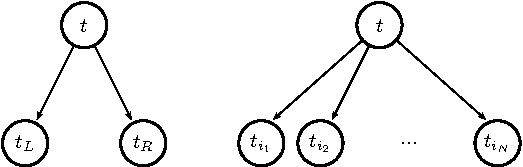
\includegraphics[scale=1.0]{figures/ch3_splits.pdf}
    \caption{Binary split of $t$ (left) and $N$-ary split of $t$ (right).}
    \label{fig:3:splits}
\end{figure}

The set ${\cal S}$ of all possible splits $s$ is the set of all partitions of
${\cal X}_t$. It is infinitely large as soon as one the input variables can
take infinitely many values. For instance, if ${\cal X}_t = \mathbb{R}$, then
there exists infinitely many ways of partitioning ${\cal X}_t$ into two (or
more) subsets. Among all of them however, only those that yield a partition of
${\cal L}_t$ into non-empty subsets are worth considering. For example, in the
binary case, splits resulting in one of the two children being empty (i.e., such
that either ${\cal L}_{t_L}$ or ${\cal L}_{t_R}$ is empty) are not considered
because their goodness cannot be evaluated on the learning set. As such, the
optimization problem of finding the best split $s^*$ of ${\cal X}_t$ can be
roughly restated as finding the best partition of the node samples ${\cal L}_t$.

Assuming distinct input values for all $N_t$ node samples, the number of partitions of ${\cal L}_t$ into $k$
non-empty subsets is given by the Stirling number of the second
kind~\citep{knuth:1992}
\begin{equation}
S(N_t, k) = \frac{1}{k!} \sum_{j=0}^k (-1)^{k-j} {k\choose j} j^{N_t},
\end{equation}
which reduces to $2^{N_t-1}-1$ for binary partitions. Given the exponential
growth in the number of partitions, the naive strategy of enumerating all
possible partitions and picking the best of them is often computationally
intractable. For this reason, simplifying  assumptions must be made on the best
split $s^*$. More specifically, the induction algorithm usually assumes that
$s^*$ -- or a least a good enough approximation -- lives in a family ${\cal Q}
\subseteq {\cal S}$ of candidate splits of restricted structure.

The usual family ${\cal Q}$ of
splits is the set of binary splits defined on a single variable and resulting
in non-empty subsets of ${\cal L}_t$:
\begin{equation}\label{eqn:q:single-variables}
{\cal Q} = \{s | s \in \bigcup_{j=1}^p {\cal Q}(X_j), {\cal L}_{t_L} \neq \phi, {\cal L}_{t_R} \neq \phi \}
\end{equation}
\begin{itemize}
\item If $X_j$ is an ordered variable taking values in ${\cal X}_j$, then the set of binary splits on $X_j$ is the set
of all binary non-crossing partitions of ${\cal X}_j$:
\begin{align}
{\cal Q}(X_j) = \{ (\{ \mathbf{x} | x_j \leq v \}, \{ \mathbf{x} | x_j > v \}) | v \in {\cal X}_j \} \label{eqn:q:ordered}
\end{align}
From a geometrical point of view, splits of this form partition the input space
${\cal X}$ with axis-parallel hyperplanes, as previously illustrated on
Figure~\ref{fig:3:partition}. Accordingly, the decision threshold $v$ thus
corresponds to the distance of the separating hyperplane from the origin.
\item If $X_j$ is a categorical variable taking values in ${\cal X}_j = \{ b_1, \dots, b_L \}$, then the set of binary splits on
$X_j$ is the set of all binary  non-empty partitions of ${\cal X}_j$:
\begin{align}\label{eqn:q:categorical-cart}
{\cal Q}(X_j) = \{ (\{\mathbf{x} | x_j \in {\cal B} \}, \{\mathbf{x} | x_j \in \overline{\cal B}\}) | &{\cal B} \subset \{ b_1, \dots, b_L \} \}
\end{align}
where $\overline{\cal B} = \{ b_1, \dots, b_L \} \setminus {\cal B}$ is the complementary set of ${\cal B}$.
\end{itemize}

Given decomposition \ref{eqn:q:single-variables} into subsets ${\cal Q}(X_j)$,
the split $s^* \in {\cal Q}$ is the best of the best splits defined on each input
variable. That is,
\begin{align}
s^* &= \argmax_{\substack{s^*_j\\ j=1, \dots, p}} \Delta i(s^*_j, t) \label{eqn:best-best-split}\\
s^*_j &= \argmax_{\substack{s \in Q(X_j)\\ {\cal L}_{t_L}, {\cal L}_{t_R} \neq \phi}} \Delta i(s, t) \label{eqn:best-split-single}
\end{align}
In this framework, the crux of the problem therefore
simply reduces to the implementation of Equation~\ref{eqn:best-split-single}.

While partitions of form~\ref{eqn:q:ordered} and \ref{eqn:q:categorical-cart}
certainly constitute the most common types of splits, alternatives proposed
over the years in the literature are worth mentioning. In ID3,
\citet{quinlan:1986} replaces binary splits on categorical variables with
exhaustive splits. That is, if ${\cal X}_j$ counts $k$ different values, then
splitting on $X_j$ divides ${\cal X}_t$ into $k$ child nodes -- one for each
value of the variable. In oblique decision trees, \citet{heath:1993} propose to
replace axis-parallel cutting hyperplanes with hyperplanes of any orientation,
resulting into smaller, yet as accurate, decision trees. In this setting
however, decomposition~\ref{eqn:best-best-split} no longer holds, hence making
the search of the best split often more computationally intensive. More
recently, several authors (e.g., \citep{gama:2004,criminisi:2013,botta:2013})
outlined more general frameworks in which splits are
defined as multi-variate functions, thereby revisiting separating hyperplanes
like in oblique trees or investigating more advanced models like quadratic
surfaces or decision trees inside decision trees. Finally, in an another
direction, several authors~\citep{adamo:1980,yuan:1995,olaru:2003} propose in fuzzy
decision trees to redefine the notion of split as overlapping fuzzy sets
(instead of disjoint subsets), hence allowing samples close to the decision
threshold $v$ to propagate into both child nodes.

\subsection{Goodness of split}
\label{sec:3:criteria}

In this section,  we describe impurity measures $i(t)$ for evaluating the
goodness of splitting rules. As they are the heart of our contributions
regarding interpretability of tree-based methods (See
Chapter~\ref{ch:importances}), the necessary mathematical foundations that have
driven their methodological development are studied here in details.
Section~\ref{sec:3:criteria:classification} reviews impurity functions for
classification while Section~\ref{sec:3:criteria:regression} discusses criteria
for regression.

\subsubsection{Classification}
\label{sec:3:criteria:classification}

Let us consider a binary classification problem defined on three binary
categorical input variables $X_1$, $X_2$ and $X_3$. Let us assume that we have
a $10$-sample learning set ${\cal L}$ as listed in Table~\ref{table:toy-problem}.
At the root node $t_0$, ${\cal L}_{t_0}$ contains all learning
samples and we are looking for the best binary split defined on one of the input
variables. Since each of them is binary and categorical, ${\cal Q}(X_j)$ (for $j=1, 2, 3$)
counts exactly one single split per input variable, each partitioning ${\cal L}_{t_0}$
into two subsets
\begin{align*}
{\cal L}_{t_L} &= \{(\mathbf{x}, y) | (\mathbf{x}, y) \in {\cal L}_{t_0}, x_j = 0\}, \\
{\cal L}_{t_R} &= \{(\mathbf{x}, y) | (\mathbf{x}, y) \in {\cal L}_{t_0}, x_j = 1\}.
\end{align*}

\begin{table}
    \centering
    \begin{tabular}{| c | c c c | c |}
    \hline
        $i$ & \textbf{$X_1$} & \textbf{$X_2$} & \textbf{$X_3$} & \textbf{$Y$} \\
    \hline
    \hline
    0 & 0 & 0 & 0 & $c_1$ \\
    1 & 0 & 0 & 1 & $c_1$ \\
    2 & 0 & 1 & 0 & $c_2$ \\
    3 & 0 & 1 & 1 & $c_2$ \\
    4 & 0 & 1 & 1 & $c_2$ \\
    5 & 1 & 0 & 0 & $c_2$ \\
    6 & 1 & 0 & 0 & $c_2$ \\
    7 & 1 & 0 & 0 & $c_2$ \\
    8 & 1 & 0 & 0 & $c_2$ \\
    9 & 1 & 1 & 1 & $c_2$ \\
    \hline
    \end{tabular}
    \captionof{table}{Toy binary classification problem}
    \label{table:toy-problem}
\end{table}

As introduced in Section~\ref{sec:3:induction}, our objective is to partition
$t_0$ using the split $s^*$ that maximizes the impurity decrease $$\Delta i(s,
t) = i(t) - p_L i(t_L) - p_R i(t_R),$$ where the impurity function $i(t)$
evaluates the goodness of node $t$. Since our goal is to build the decision
tree that minimizes generalization error, it seems natural to take as proxy
$i(t)$ the local resubstitution estimate at node $t$:
\begin{definition}
In classification, the impurity function $i_R(t)$ based on the local resubstitution estimate
defined on the zero-one loss is:
\begin{equation}\label{eqn:impurity:error}
i_R(t) = 1 - p(\widehat{y}_t|t) =  1 - \max_{c \in {\cal Y}} p(c|t)
\end{equation}
\end{definition}
With this criterion, selecting the best split would amount to pick the split that most
decreases training error. In spite of its natural attractiveness however,
$i_R(t)$ has two serious defects:
\begin{enumerate}
\item As a corollary of Proposition~\ref{prop:any-split-reduce-classification},
      $\Delta i(s, t)$ is zero for all splits if the majority class remains
      the same in both child nodes, that is if $\widehat{y}_t = \widehat{y}_{t_L} = \widehat{y}_{t_R}$.

      In our toy problem, splitting either on $X_1$, $X_2$ or $X_3$ produces
      child nodes in which the majority class remains class $1$. As a result,
      $\Delta i(s, t_0) = 0$ for all three possible splits, as if they were
      equally bad, or as if no further improvement could be achieved.

\item It does not sensitively account for changes in the a posteriori class
      distributions $p(y|t_L)$ and $p(y|t_R)$.

      In our example, none of the three splits improves training error. However,
      splitting on $X_1$ is likely to yield a tree which is simpler than if the
      root node had been split on $X_3$.  As shown in
      Figure~\ref{fig:3:goodness}, splitting on $X_1$ indeed produces a child
      node that is already terminal and for which no further work is required.
      By contrast, splitting on $X_3$ results in child nodes that still have to be
      divided further.  Splitting on $X_1$ should therefore be preferred, even
      if it does not reduce immediately the training error.
\end{enumerate}

\begin{figure}[h]
    \centering
    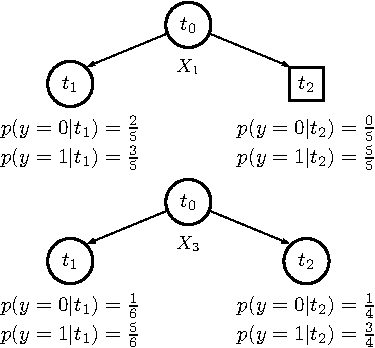
\includegraphics[scale=1.0]{figures/ch3_goodness.pdf}
    \caption{Splitting on $X_1$ versus splitting on $X_3$.}
    \label{fig:3:goodness}
\end{figure}

In fact, these issues are largely due to the fact that the tree growing
algorithm~\ref{algo:induction} is based on a one-step optimization procedure. A
good impurity criterion should ideally also take into account the possibility
of further improvement deeper in the tree. To avoid the undesirable properties
of $i_R(t)$, the choice of $i(t)$ should therefore be
guided by ensuring that $i(t)$ gets progressively smaller when $t$ gets more
homogeneous towards one (or some) of the classes (while not being necessarily
better in terms of misclassification error) and larger when $t$ is more
heterogeneous. In CART, \citet{breiman:1984} identify a class of impurity
function $i(t)$ meeting these requirements:

\begin{theorem}\label{thm:reduction-impurity}
Let $\Phi(p_1, \dots, p_J)$ be a strictly concave $J$-ary function defined
on $0 \leq p_k \leq 1$, for $k=1,\dots,J$, $\sum_{k=1}^J p_k = 1$ and such that
\begin{itemize}
\item $\Phi(1, \dots, 0) = \Phi(0, 1, \dots, 0) = \dots = \Phi(0, \dots, 1)$ is minimal;
\item $\Phi(\frac{1}{J}, \dots, \frac{1}{J})$ is maximal.
\end{itemize}
Then, for $i(t) = \Phi(p(c_1|t), \dots, p(c_J|t))$ and any split $s$, $$\Delta i(s, t) \geq 0,$$
with equality if and only if $p(c_k|t_L)=p(c_k|t_R)=p(c_k|t)$ for $k=1,\dots,J$.
\end{theorem}

\begin{proof}
Let us first remark that
\begin{align*}
p_L p(c_k|t_L) + p_R p(c_k|t_R) &= \frac{N_{t_L}}{N_t} \frac{N_{c_kt_L}}{N_{t_L}} +  \frac{N_{t_R}}{N_t} \frac{N_{c_kt_R}}{N_{t_R}} \\
                                &= \frac{N_{c_kt_L} + N_{c_kt_R}}{N_t} \\
                                &= \frac{N_{c_kt}}{N_t} \\
                                &= p(c_k|t)
\end{align*}
By strict concavity, it comes
\begin{align*}
p_L i(t_L) + p_R i(t_R) &= p_L \Phi(p(c_1|t_L), \dots, p(c_J|t_L)) + p_R \Phi(p(c_1|t_R), \dots, p(c_J|t_R)) \\
                        &\leq \Phi(p_L p(c_1|t_L) + p_R p(c_1|t_R), \dots, p_L p(c_J|t_L) + p_R p(c_J|t_R)) \\
                        &= \Phi(p(c_1|t), \dots, p(c_J|t)) \\
                        &= i(t)
\end{align*}
with equality if and only
if $p(c_k|t_L)=p(c_k|t_R)$ for $k=1,\dots,J$.
\end{proof}

\begin{figure}
\centering
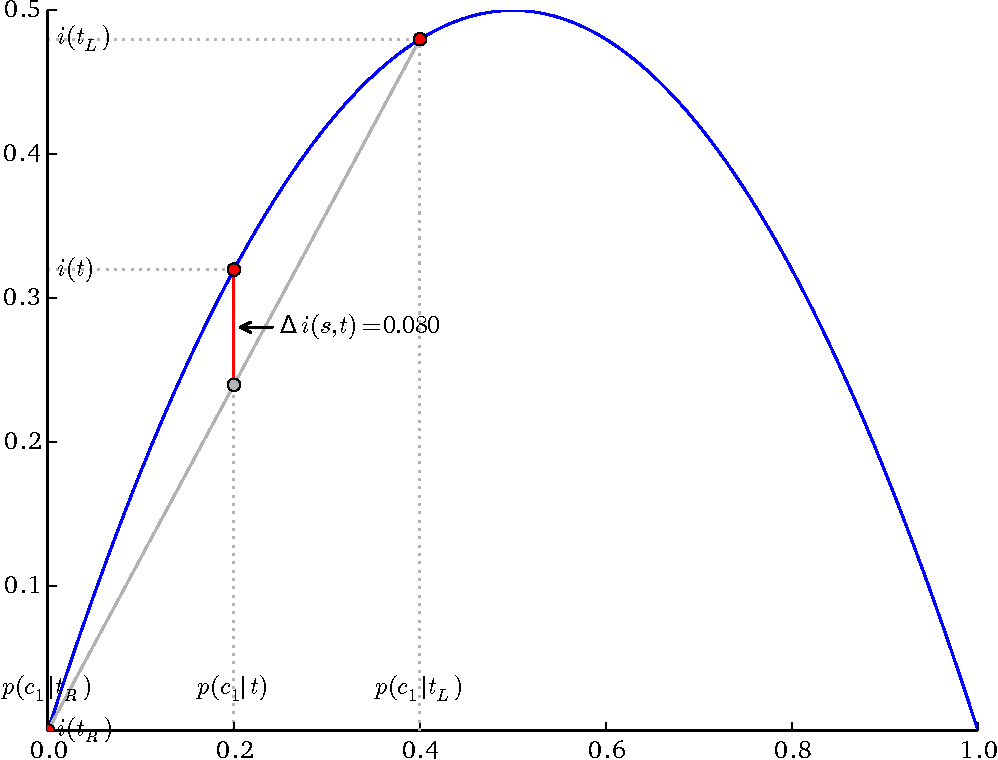
\includegraphics[width=0.9\textwidth]{figures/ch3_toy_x1_gini.pdf}\\
\vspace{1cm}
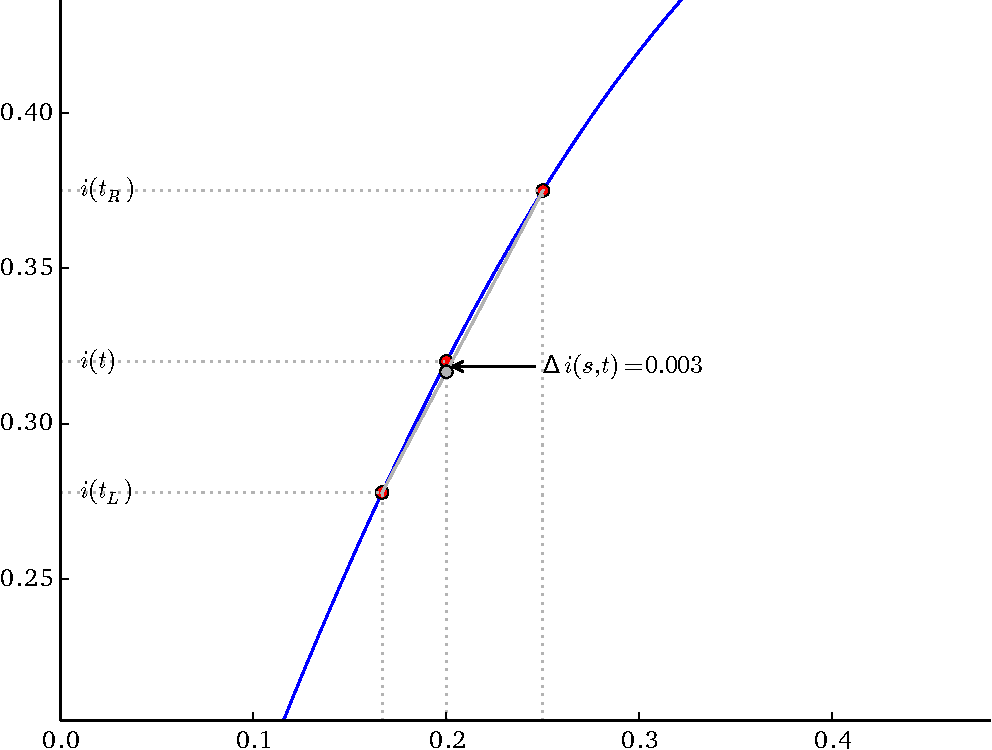
\includegraphics[width=0.9\textwidth]{figures/ch3_toy_x3_gini.pdf}
\caption{Splitting $t_0$ on $X_1$ (above) versus splitting $t_0$ on $X_3$ (below), as evaluated by a strictly concave impurity function.}
\label{fig:3:toy:impurity:gini}
\end{figure}

To better understand Theorem~\ref{thm:reduction-impurity}, let us consider a
strictly concave function $\Phi$ that satisfies the requirements and let us
evaluate on our toy problem the goodness of the split defined on $X_1$.  As
illustrated in the first plot of Figure~\ref{fig:3:toy:impurity:gini},  $i(t)$
is maximum when the uncertainty on the output value is the largest
(i.e., at $p(c_1|t)=p(c_2|t)=\tfrac{1}{2}$) and then gets progressively smaller
when certainty grows towards one of the classes (i.e., as $p(c_1|t)$
gets close to $0$ or $1$). As shown by Theorem~\ref{thm:reduction-impurity},
$i(t)$ is also necessarily larger than the weighted sum (illustrated by the gray
dot) of impurities of the child nodes. Visually, the further away $p(c_1|t_L)$
and $p(c_1|t_R)$ from $p(c_1|t)$, the larger $\Delta i(s,t)$ (illustrated by
the red line) and the better the split $s$. By contrast, when $s$ does not
significantly change the a posteriori class distributions, as illustrated in
the second plot of Figure~\ref{fig:3:toy:impurity:gini} when splitting $t_0$ on
$X_3$, then the closer $p(c_1|t_L)$ and $p(c_1|t_R)$ from $p(c_1|t)$ and the
smaller $\Delta i(s,t)$. Yet, as long as the a posteriori class distributions
do not exactly coincide with the a priori class distribution, then even the
slightest changes get captured by $\Delta i(s, t)$ because of strict concavity.
It is only when they exactly coincide (i.e., when
$p(c_1|t_L)=p(c_1|t_R)=p(c_1|t)$) that the three red points overlap and that
$\Delta i(s,t)=0$.

\begin{figure}
\centering
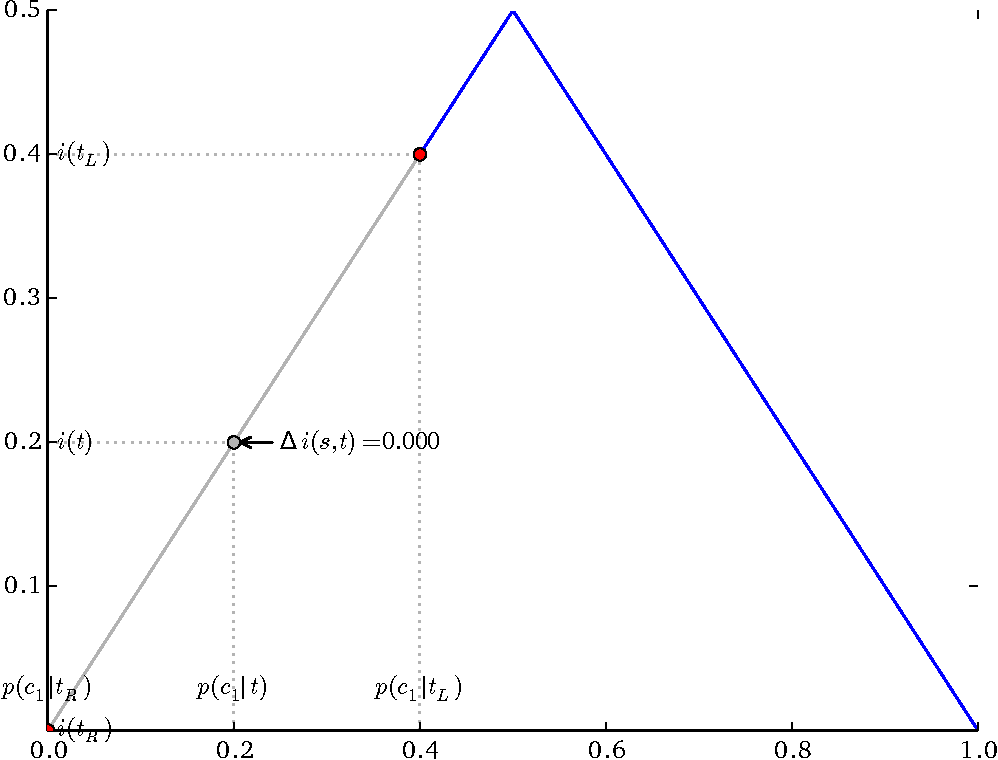
\includegraphics[width=0.9\textwidth]{figures/ch3_toy_x1_error.pdf}
\caption{Splitting $t_0$ on $X_1$ as evaluated by the resubstitution estimate $i_R(t)$.}
\label{fig:3:toy:impurity:error}
\end{figure}

Graphically, it also becomes obvious when comparing
Figure~\ref{fig:3:toy:impurity:gini} with Figure~\ref{fig:3:toy:impurity:error}
to understand why the resubstitution estimate $i_R(t)$ is not an appropriate
impurity function. As long as the majority class within the child nodes $t_L$
and $t_R$ is the same as in $t$, the three red dots remain aligned in a perfect
line and the gray dot overlap with $i(t)$. As a result, $\Delta i(s,t)$ is
necessarily null no matter the a posteriori class distributions induced by the
split, be them close or far from $p(c_1|t)$.

The most common impurity criteria used for classification trees are the Shannon
entropy and the Gini index:

\begin{definition}
The impurity function $i_H(t)$ based on the Shannon entropy~\citep{shannon:1949} is:
\begin{equation}\label{eqn:impurity:shannon}
i_H(t) = - \sum_{k=1}^J p(c_k|t) \log_2 (p(c_k|t))
\end{equation}
\end{definition}
\begin{definition}
The impurity function $i_G(t)$ based on the Gini index~\citep{gini:1912} is:
\begin{equation}\label{eqn:impurity:gini}
i_G(t) = \sum_{k=1}^J p(c_k|t) (1 - p(c_k|t))
\end{equation}
\end{definition}

As illustrated on Figure~\ref{fig:3:toy:impurity:comparison}, both $i_H(t)$ and
$i_G(t)$ satisfy the requirements of Theorem~\ref{thm:reduction-impurity} and
exhibit the properties that we are looking for. The entropy-based impurity
$i_H(t)$ quantifies the uncertainty of $Y$ within node $t$. With this
criterion, the impurity decrease $\Delta i_H(s,t)$, also known as the
\textit{information gain}, represents the information learned about
$Y$ by splitting $t$ into $t_L$ and $t_R$. The Gini-based impurity $i_G(t)$
measures how often a randomly chosen object $\mathbf{x}\in {\cal L}_t$ would be
incorrectly classified if it were randomly labeled by a class $c\in{\cal Y}$ according
to the distribution $p(y|t)$.

\begin{figure}
\centering
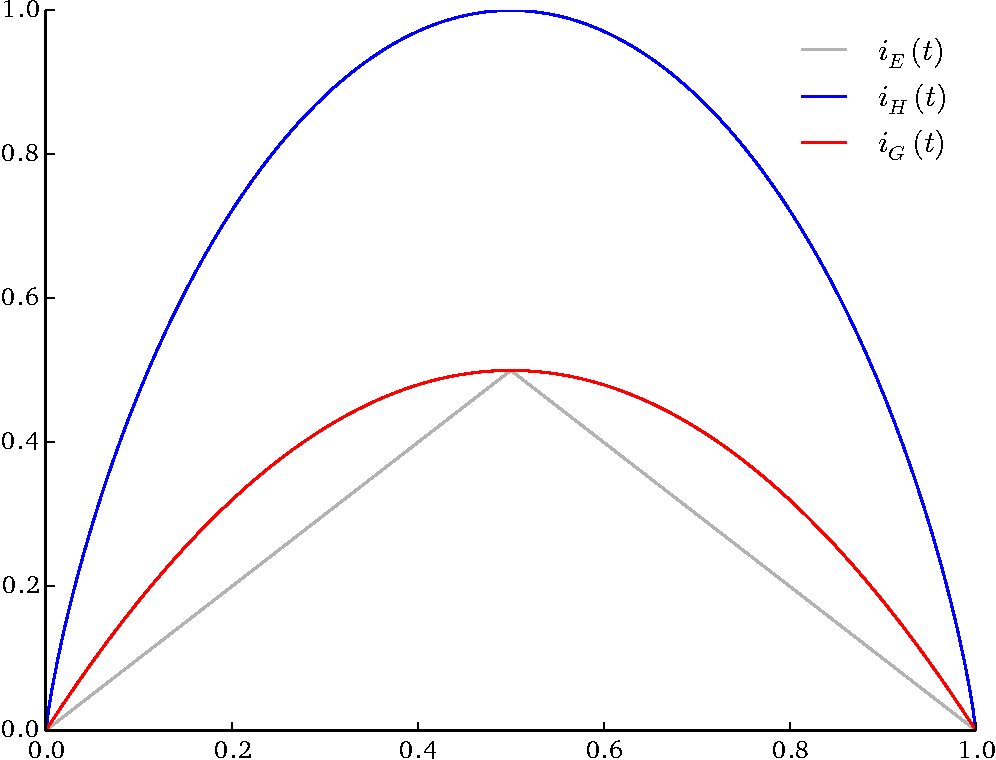
\includegraphics[width=0.9\textwidth]{figures/ch3_impurity_comparison.pdf}
\caption{Comparison of $i_E(t)$, $i_H(t)$ and $i_G(t)$.}
\label{fig:3:toy:impurity:comparison}
\end{figure}

While the Shannon entropy~\ref{eqn:impurity:shannon} and the Gini
index~\ref{eqn:impurity:gini} are robust and reliable impurity functions
usually producing accurate decision trees, they are not exempt of defects. One
of the most well-known issues is end-cut
preference~\citep{morgan:1973,breiman:1984}, that is the tendency to favor
unbalanced splits in which $p_L$ is close to zero or one,  often resulting in
deep and uninterpretable decision trees. Another defect is the propensity of
preferring splits based on input variables with many outcomes rather than
selecting input variables without bias with respect to their
cardinality~\citep{quinlan:1986,strobl:2007}. Intuitively, if $|{\cal X}_1| >
|{\cal X}_2|$ and that both $X_1$ and $X_2$ are independent of $Y$, then $X_1$
is indeed more likely to be selected than $X_2$  because of chance. To overcome
these issues, numerous variants of impurity measures have been proposed in the
literature, including normalization techniques, distance-based measures or
causality-based impurity functions (see
\citep{wehenkel:1996,zighed:2000,maimon:2005} for reviews on the topic). From
an empirical point of view however,  several
studies~\citep{mingers:1989b,miyakawa:1989,mantaras:1991} have shown that,
while the impurity function may have a significant impact on the structure of
the decision tree, improvements in terms of classification accuracy are usually
not that significant.

\subsubsection{Regression}
\label{sec:3:criteria:regression}

When the output variable $Y$ is quantitative, Proposition~\ref{prop:any-split-reduce-regression}
shows that splitting $t$ in any way reduces the
square error loss on the training set. In particular, the reduction is positive as long as
the values assigned to the child nodes are different from the value at $t$.
Contrary to classification, this only happens in rare circumstances (i.e., when
the mean output values at the child nodes coincide with the mean output value
in $t$), hence making the regression resubstitution estimate sensitive to changes in the a
posteriori distributions, even if these are only slight.  As a result, the
local resubstitution estimate does not exhibit the undesirable properties that
we had in classification and in fact constitutes a good criterion for
regression.

\begin{definition}
In regression, the impurity function $i_R(t)$ based on the local resubstitution estimate
defined on the square error loss is:
\begin{equation}\label{eqn:impurity:variance}
i_R(t) = \frac{1}{N_t} \sum_{\mathbf{x}, y \in {\cal L}_t} (y - \widehat{y}_t)^2
\end{equation}
\end{definition}

Another way of looking at criterion~\ref{eqn:impurity:variance} is to notice
that it corresponds to the within node variance of the output value in $t$.
Accordingly, $s^*$ is the split that maximizes the reduction of variance
$\Delta i(s, t)$ in the child nodes.

\begin{remark}{Equivalence between classification and regression trees}
When ${\cal Y} = \{0, 1\}$, the learning problem can either be
stated as a binary classification task where $c_1=0$ and $c_2=1$ or as a regression
task where the goal is to predict the most accurate predictions $\widehat{y} \in {\cal Y} \subseteq \mathbb{R}$.
Interestingly, regression trees built in this setting are in fact strictly
equivalent to classification trees built using the Gini index $i_G(t)$. Indeed since $\widehat{y}_t = \tfrac{1}{N_t} \sum_{\mathbf{x}, y \in {\cal L}_t} y = p(c_2|t) = 1 - p(c_1|t)$, it comes:
\begin{align}
i_R(t) &= \frac{1}{N_t} \sum_{\mathbf{x}, y \in {\cal L}_t} (y - \widehat{y}_t)^2 \nonumber \\
       &= \frac{1}{N_t} \sum_{\mathbf{x}, y \in {\cal L}_t} y - 2 y \widehat{y}_t + \widehat{y}_t^2 \nonumber \\
       &= \widehat{y}_t - 2 \widehat{y}_t^2 + \widehat{y}_t^2 \nonumber \\
       &= \widehat{y}_t (1 - \widehat{y}_t) \nonumber \\
       &= p(c_2|t) (1 - p(c_2|t)) \nonumber \\
       &= \frac{1}{2} i_G(t)
\end{align}
From a practical point of view, this means that both classification and
regression trees could be implemented using the single criterion~\ref{eqn:impurity:variance}.
\end{remark}

\subsection{Finding the best binary split}

Now that we have described families ${\cal Q}$ of splitting rules and impurity
criteria to evaluate their respective goodness, the last thing which is missing
to have a complete specification of the induction
algorithm~\ref{algo:induction} is an efficient optimization procedure for
finding the best split $s^* \in {\cal Q}$. Assuming that ${\cal Q}$ is the set
of binary univariate splits, we showed in Section~\ref{sec:3:splitting-rules:families}
that $s^*$ is the best of the best binary splits $s^*_j$
defined on each input variable. This leads to the following procedure:

\begin{algorithm}\label{algo:findsplit}
Find the best split $s^*$ that partitions ${\cal L}_t$.
\textnormal{
\begin{algorithmic}[1]
\Function{FindBestSplit}{${\cal L}_t$}
    \State $\Delta = -\infty$
    \For{$j=1, \dots, p$}
        \State Find the best binary split $s^*_j$ defined on $X_j$
        \If{$\Delta i(s^*_j, t) > \Delta$}
            \State $\Delta = \Delta i(s^*_j, t)$
            \State $s^* = s^*_j$
        \EndIf
    \EndFor
    \State \Return $s^*$
\EndFunction
\end{algorithmic}
}
\end{algorithm}

\subsubsection{On an ordered variable}
\label{sec:best-split-ordered}

Let $X_j$ be an ordered variable and let ${\cal Q}(X_j)$ be the set of all
binary non-crossing partitions of ${\cal X}_j$, as defined in
Equation~\ref{eqn:q:ordered}. Let also ${\cal X}_{j|{\cal L}_t} = \{ x_j | \mathbf{x},y
\in {\cal L}_t \}$ denotes the set of unique values of $X_j$ within the node
samples in $t$.  The best split on $X_j$ is the best binary partition
$s^v_j \in {\cal Q}(X_j)$ of ${\cal L}_t$ into two non-empty subsets:
\begin{align*}
{\cal L}^v_{t_L} &= \{(\mathbf{x}, y)|(\mathbf{x}, y)\in {\cal L}_t, x_j \leq v\}\\
{\cal L}^v_{t_R} &= \{(\mathbf{x}, y)|(\mathbf{x}, y)\in {\cal L}_t, x_j > v\}
\end{align*}
where $v$ is the decision threshold of the split. As illustrated in
Figure~\ref{fig:3:split-ordered}, there exist $|{\cal X}_{j|{\cal
L}_t}|-1$ partitions of ${\cal L}_t$ into two such non-empty subsets, i.e., one
for each value $v_k \in {\cal X}_{j|{\cal L}_t}$, except for the last one which
leads to an invalid partition. In particular, if $X_j$ is locally constant in
$t$ (i.e., if all dots overlap in Figure~\ref{fig:3:split-ordered}), then
$|{\cal X}_{j|{\cal L}_t}|=1$ and $X_j$ cannot be used to partition $t$. More
importantly, there usually exist several thresholds $v$ producing the same
partition of the node samples. If $v_k$ and $v_{k+1}$ are two immediately
consecutive values in  ${\cal X}_{j|{\cal L}_t}$, then all splits $s^{v}_j$ for
$v \in [v^k, v^{k+1}[$ indeed produce the same partition of ${\cal L}_t$ as
$s^{v_k}_j$ does. In terms of impurity decrease $\Delta i$, all of them are
thus equivalent when evaluated on ${\cal L}_t$. In generalization however,
these splits may not be strictly the same since they do not produce the same
partition of ${\cal X}_t$. As a compromise, the decision thresholds that are
thus usually chosen are the mid-cut-points $v^\prime_k=\tfrac{v_k+v_{k+1}}{2}$
between consecutive values of the variable, as shown by the dotted line in
Figure~\ref{fig:3:split-ordered}. In practice, this is indeed a good-enough
heuristic on most problems.

\begin{figure}
    \centering
    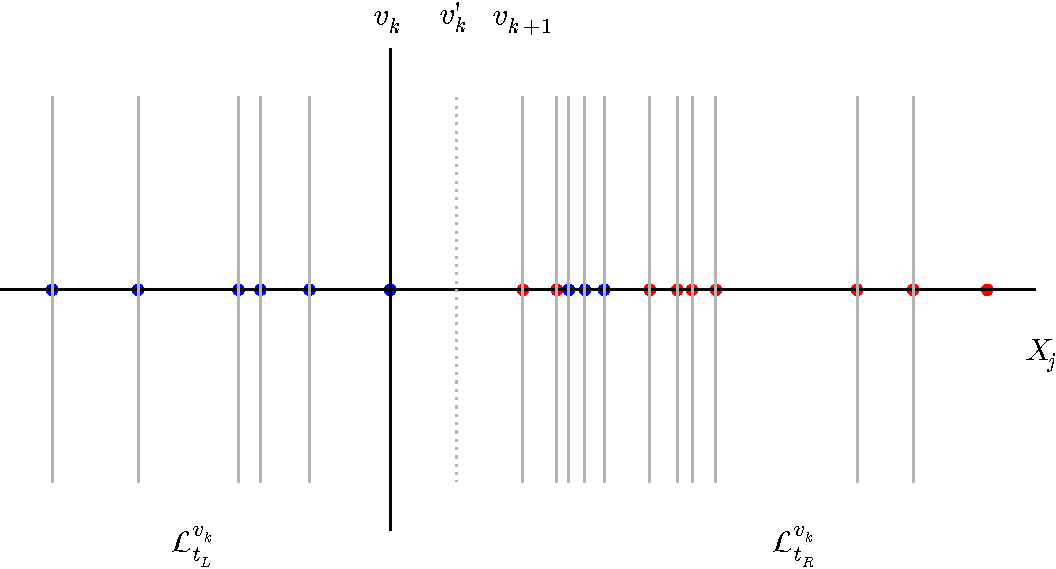
\includegraphics[width=0.9\textwidth]{figures/ch3_split_ordered.pdf}
    \caption{Binary partitions of ${\cal L}_t$ on the ordered variable $X_j$. Setting the decision threshold $v$ to any value in $[v_k;v_{k+1}[$ yields identical partitions of ${\cal L}_t$, but not of ${\cal X}_t$.}
    \label{fig:3:split-ordered}
\end{figure}

In this framework, the best split $s^*_j$ is the split
$\smash{s^{v^\prime_k}_j}$ that maximizes impurity decrease. Computationally,
the exhaustive evaluation of all these splits can be carried out efficiently when
considering decision thresholds $v^\prime_k$ in sorted order, by remarking that
$\smash{\Delta i(s^{v^\prime_{k+1}}_j, t)}$ can be computed  from
$\smash{\Delta i(s^{v^\prime_{k}}_j, t)}$ in a limited number of operations.

\begin{itemize}

\item In classification, evaluating either $\Delta i_H(s, t)$ or $\Delta i_G(s, t)$
      boils down to the computation of $p(c|t)$, $p(c|t_L)$ and $p(c|t_R)$
      for all classes $c \in {\cal Y}$. The necessary statistics for computing
      these probabilities are the numbers $N_{ct}$, $N_{ct_L}$ and $N_{ct_R}$
      of samples of class $c$ in $t$, $t_L$ and $t_R$, along with the total numbers
      $N_t$, $N_{t_L}$ and $N_{t_R}$ of samples in $t$, $t_L$ and $t_R$.
      $N_{ct}$ and $N_t$ can be computed once for all splits.
      The four other statistics can be computed iteratively, from
      $\smash{s^{v_k^\prime}_j}$ to $\smash{s^{v_{k+1}^\prime}_j}$:
      \begin{align}
      N_{t_L}^{v^\prime_{k+1}} &= N_{t_L}^{v^\prime_{k}} + |\{ (\mathbf{x},y) | (\mathbf{x},y) \in {\cal L}^{v^\prime_{k+1}}_{t_L} \cap {\cal L}^{v^\prime_{k}}_{t_R} \}| \label{eqn:criterion:n_tl} \\
      N_{ct_L}^{v^\prime_{k+1}} &= N_{ct_L}^{v^\prime_{k}} + |\{ (\mathbf{x},y) | (\mathbf{x},y) \in {\cal L}^{v^\prime_{k+1}}_{t_L} \cap {\cal L}^{v^\prime_{k}}_{t_R}, y=c \}| \\
      N_{t_R}^{v^\prime_{k+1}} &= N_{t_R}^{v^\prime_{k}} - |\{ (\mathbf{x},y) | (\mathbf{x},y) \in {\cal L}^{v^\prime_{k+1}}_{t_L} \cap {\cal L}^{v^\prime_{k}}_{t_R} \}| \label{eqn:criterion:n_tr} \\
      N_{ct_R}^{v^\prime_{k+1}} &= N_{ct_R}^{v^\prime_{k}} - |\{ (\mathbf{x},y) | (\mathbf{x},y) \in {\cal L}^{v^\prime_{k+1}}_{t_L} \cap {\cal L}^{v^\prime_{k}}_{t_R}, y=c \}|
      \end{align}
      where ${\cal L}^{v^\prime_{k+1}}_{t_L} \cap {\cal
      L}^{v^\prime_{k}}_{t_R}$ are the node samples going from the right child
      node to the left child node when switching from
      $\smash{s^{v_k^\prime}_j}$ to $\smash{s^{v_{k+1}^\prime}_j}$.

\item In regression, $i_R(t)$ can be re-expressed as the difference between the
      mean of the squared output values and the square of the mean output value, that is
      \begin{equation}
      i_R(t) = \frac{\Sigma_{t^2}}{N_t} - (\frac{\Sigma_t}{N_t})^2
      \end{equation}
      where $\Sigma_t = \sum_{\mathbf{x}, y \in {\cal L}_t} y$ and $\Sigma_{t^2}
      = \sum_{\mathbf{x}, y \in {\cal L}_t} y^2$. In this form, the necessary
      statistics for computing $\Delta i_R(s, t)$ are $\Sigma_t$, $\Sigma_{t^2}$,
      $\Sigma_{t_L}$, $\Sigma_{t_L^2}$, $\Sigma_{t_R}$ and $\Sigma_{t_R^2}$, along with the total numbers
      $N_t$, $N_{t_L}$ and $N_{t_R}$ of samples in $t$, $t_L$ and $t_R$. As in classification,
      $\Sigma_t$, $\Sigma_{t^2}$ and $N_t$ can be computed once for all splits, while $N_{t_L}$ and $N_{t_R}$
      can be computed from one split to another using Equations~\ref{eqn:criterion:n_tl} and \ref{eqn:criterion:n_tr}.
      The four other statistics can be computed iteratively, from
      $\smash{s^{v_k^\prime}_j}$ to $\smash{s^{v_{k+1}^\prime}_j}$:
      \begin{align}
      \Sigma_{t_L}^{v^\prime_{k+1}} &= \Sigma_{t_L}^{v^\prime_{k}} + \sum_{(\mathbf{x},y) \in {\cal L}^{v^\prime_{k+1}}_{t_L} \cap {\cal L}^{v^\prime_{k}}_{t_R}} y \\
      \Sigma_{t_L^2}^{v^\prime_{k+1}} &= \Sigma_{t_L^2}^{v^\prime_{k}} + \sum_{(\mathbf{x},y) \in {\cal L}^{v^\prime_{k+1}}_{t_L} \cap {\cal L}^{v^\prime_{k}}_{t_R}} y^2 \\
      \Sigma_{t_R}^{v^\prime_{k+1}} &= \Sigma_{t_R}^{v^\prime_{k}} - \sum_{(\mathbf{x},y) \in {\cal L}^{v^\prime_{k+1}}_{t_L} \cap {\cal L}^{v^\prime_{k}}_{t_R}} y \\
      \Sigma_{t_R^2}^{v^\prime_{k+1}} &= \Sigma_{t_R^2}^{v^\prime_{k}} - \sum_{(\mathbf{x},y) \in {\cal L}^{v^\prime_{k+1}}_{t_L} \cap {\cal L}^{v^\prime_{k}}_{t_R}} y^2
      \end{align}

\end{itemize}

Starting from the initial partition $v^\prime_0=-\infty$, that is where $t_L$
is empty and $t_R$ corresponds to $t$, and using the above update equations to
switch from $\smash{v^\prime_k}$ to $\smash{ v^\prime_{k+1}}$, the search of
best split $s^*_j$ on $X_j$ can be implemented as described in
Algorithm~\ref{algo:findsplit:x_j} and further illustrated in
Figure~\ref{fig:3:split:invariant}.

\begin{algorithm}\label{algo:findsplit:x_j}
Find the best split $s^*_j$ on $X_j$ that partitions ${\cal L}_t$.
\textnormal{
\begin{algorithmic}[1]
\Function{FindBestSplit}{${\cal L}_t$, $X_j$}
    \State $\Delta = 0$
    \State $k = 0$
    \State $v^\prime_k = -\infty$
    \State Compute the necessary statistics for $i(t)$
    \State Initialize the statistics for $t_L$ to $0$
    \State Initialize the statistics for $t_R$ to those of $i(t)$
    \State Sort the node samples ${\cal L}_t$ such that $x_{1,j} \leq x_{2, j} \leq \dots \leq x_{N_t,j}$
    \State $i = 1$
    \While{$i \leq N_t$}
        \While{$i + 1 \leq N_t$ and $x_{i+1,j} = x_{i,j}$}
            \State $i = i + 1$
        \EndWhile{}
        \State $i = i + 1$
        \If{$i \leq N_t$}
            \State $v^\prime_{k+1} = \tfrac{x_{i,j} + x_{i-1,j}}{2}$
            \State Update the necessary statistics from $v^\prime_k$ to $v^\prime_{k+1}$
            \If{$\smash{\Delta i(s^{v^\prime_{k+1}}_j, t) > \Delta}$}
                \State $\smash{\Delta = \Delta i(s^{v^\prime_{k+1}}_j, t)}$
                \State $s^*_j = s^{v^\prime_{k+1}}_j$
            \EndIf{}
            \State $k = k+1$
        \EndIf{}
    \EndWhile{}
    \State \Return $s^*_j$
\EndFunction
\end{algorithmic}
}
\end{algorithm}

\begin{figure}[h]
    \centering
    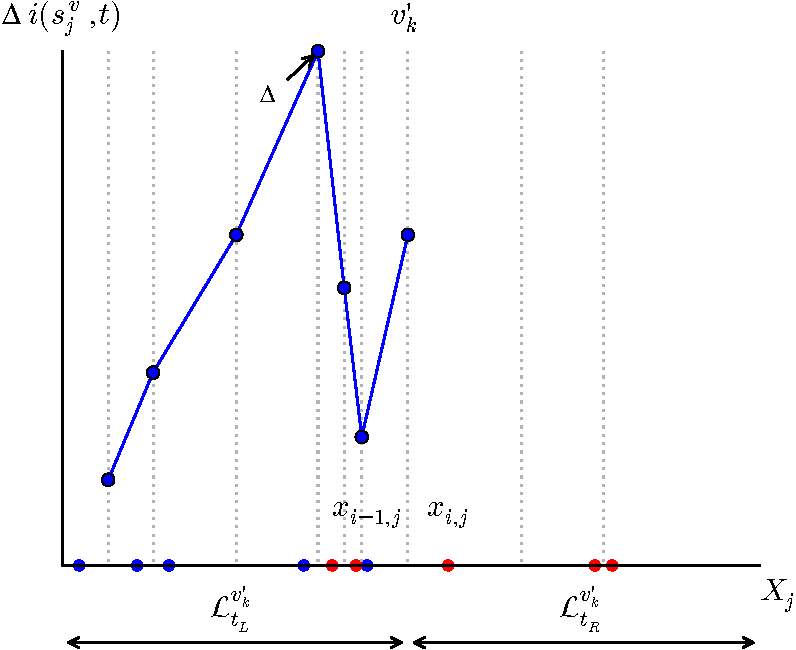
\includegraphics[width=0.9\textwidth]{figures/ch3_split_ordered_invariant.pdf}
    \caption{Loop invariant of Algorithm~\ref{algo:findsplit:x_j}. At the end of each
    iteration, $\smash{\Delta i(s^{v^\prime_k}_j, t)}$ has been computed from the
    statistics of the previous split at $v^\prime_{k-1}$  and compared to the
    best reduction in impurity $\Delta$ found so far within the splits at $v^\prime_{0}=-\infty$ to $v^\prime_{k-1}$.}
    \label{fig:3:split:invariant}
\end{figure}

As we will see later in
Chapter~\ref{ch:complexity}, the algorithm complexity is upper bounded by the
complexity of the sorting operation. In the context of randomized decision
trees however, where finding the very best split $s^*_j$ is not as crucial, we
will show that approximation techniques based on sub-sampling of the node
samples or on the discretization of the variable $X_j$ can help reduce the
computational complexity of procedure without significant impact on accuracy.

% \subsection{Approximately best binary split on an ordered variable}
% \label{sec:best-split-ordered-approx}

%             + Binning
%             + Subsampling


\subsubsection{On a categorical variable}
\label{sec:best-split-categorical}

Let $X_j$ be a categorical variable and let ${\cal Q}(X_j)$ be the set of all
binary partitions of ${\cal X}_j= \{ b_1, \dots, b_L \}$, as defined in
Equation~\ref{eqn:q:categorical-cart}. The number of non-empty binary
partitions in this set is $2^{L-1}-1$, which may quickly become highly
prohibitive to  explore exhaustively when $X_j$ counts a high number $L$
of categories.

Fortunately, in binary classification, this exponential complexity can be
reduced from looking at $2^{L-1}-1$ partitions to $L-1$ partitions, thanks a
theoretical result due to \citet{fisher:1958} and \citet{breiman:1984}:
\begin{theorem}\label{thm:categorical-simplification}
Let reorder the categories of $X_j$ such that
$$p(c_1|t,X_j=b_{l_1}) \leq p(c_1|t,X_j=b_{l_2}) \leq \dots \leq p(c_1|t,X_j=b_{l_L}).$$
If the impurity function $i(t)$ satisfies the requirements of Theorem~\ref{thm:reduction-impurity}, then one
of the $L-1$ subsets ${\cal B}=\{b_{l_1}, \dots, b_{l_h}\}, h=1, \dots, L-1$ defines
a binary partition of the node samples into
\begin{align*}
{\cal L}^{\cal B}_{t_L} &= \{(\mathbf{x}, y)|(\mathbf{x}, y)\in {\cal L}_t, x_j \in {\cal B}\}\\
{\cal L}^{\cal B}_{t_R} &= \{(\mathbf{x}, y)|(\mathbf{x}, y)\in {\cal L}_t, x_j \in \overline{{\cal B}}\}
\end{align*}
which maximizes $\Delta i(s, t)$, for $s \in {\cal Q}(X_j)$.
\end{theorem}
Intuitively, this result indicates that all those categories $b_l$ leading to
high probabilities of being of class $c_1$ should be put together into one node
and the categories leading to lower probabilities into the other. In practice,
this also means that the search of the best binary split can be performed as if
$X_j$ was an ordered variable, by virtually replacing categorical values $b_l$
with $p(c_1|t,X_j=b_l)$ and using Algorithm~\ref{algo:findsplit:x_j} to find
the best binary split on these ordered values.

Unfortunately, Theorem~\ref{thm:categorical-simplification} does not extend to
multi-class classification (i.e., when $J > 2$). In this case, an exhaustive
exploration of all $2^{L-1}-1$ splits must be performed in order
to find the best split.  When the number $L$ of categories is small, this can
usually be done  within reasonable time. However, as $L$ gets larger, this
quickly becomes infeasible in practice. As an approximation, the usual
strategy~\citep{liaw:2002} consists in exhaustively evaluating all splits when
$L \leq 10$ and then switch to random sampling of the subsets ${\cal B} \subset
\{ b_1, \dots, b_L \}$ when $L > 10$. In that case, $512$ random subsets ${\cal
B}$ are typically drawn and evaluated.

In regression, given the equivalence of $i_R(t)$ with the Gini index, the same
algorithmic trick can be applied as in binary classification. In this case,
$X_j$ is transformed into an ordered variable by virtually replacing
categorical values $b_l$ with the mean output value at $b_l$, i.e.,
$\tfrac{1}{N_{lt}} \sum_{\mathbf{x}, y \in {\cal L}_t, x_j = b_l} y$, on which
Algorithm~\ref{algo:findsplit:x_j} is then applied to find the best binary
split on these ordered values.


\section{Multi-output trees}

\todo{}

% multi-objective regression trees
% https://dtai.cs.kuleuven.be/clus/publications.html

% présentation
% structured learning
% output kernel tree
